\begin{intersong}
    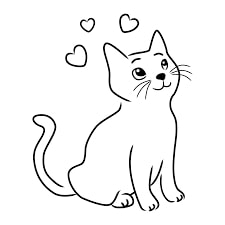
\includegraphics[width=0.4\textwidth]{diekatkomweer}
\end{intersong}
\beginsong{Die kat kom weer}
\beginverse
Die boer die zwoer hem blau: hij zou die kat doodskiet,
hij heeft die roer gelaän met kruid en dynamiet;
Hij lei hem op de weg waardoor die kat moes kom;
Haren en velletjes en beentjes.
\endverse
\beginchorus
Maar die kat kom weer, die kon nie langer wach,
die kat kom weer, die volgende dag.
Die kat kom weer, geloof me het is waar,
die volgende dag is die kat weer daar.
\endchorus
\beginverse
Hij zet hem op een skip, die zeilde naar Japan,
die skip was gelaän met twalefhonderd man.
Maar verre van die land, daar is die skip gestrand;
En alle passagiers verdronken.
\endverse
\beginverse
Die boer die zat die kat in een aëroplaan,
die botste eventjes tegen een wolkie aan.
Die boel die viel omlaag, bleef teken in een haag!
Alleman brak nek en benen.
\endverse
\beginverse
Die boer die bond die kat die pootjes netjes saam,
en lei die beesjie op de railtjes van de tram.
Die trampie liep van spoor, en brak te midden door:
stukken glas en hout en ijzer!
\endverse
\beginverse
Toen kap die boer die kat in duizend stuk kif kaf, 
en steek dan ieder stuk apaartjes in’n graf.
Hij stamp die boel goed aan en dank: het is gedaan.
Maar als hij sliep dan droomde hij altijd. 
\endverse
\endsong